	\chapter{Hjertesykdommer}
			\chapterprecishere{40 \% av alle nordmenn dør av hjerte- karsykdommer\raggedleft--- \textup{Statistisk sentralbyrå, Dødsårsaksregisteret\\[0.5in]}}
		
		\section{Perlene...}
			\begin{itemize}
				\item Hjertesvikt er ikke en egen sykdom men en beskrivelse av nedsatt hjertefunksjon.\\
				\item NYHA beskriver hvor alvorlig hjertesvikten er og er basert på hvordan pasientene fungerer i hverdagen.\\
				\item Hjertesvikt har høy dødelighet.\\
				\item De eldste, kvinner og pasienter med diabetes har ofte helt utypiske symptomer på hjerteinfarkt.\\
				\item Digitalis har lang halveringstid i kroppen.\\
				\item Diare og slapphet er vanligste symptomer ved digitalisoverdose.\\
				\item Digitalis brukes i behandling av atrieflimmer for å stabiliserer hjerterytmen.\\
			\end{itemize}

		\section{Noen sykdommer av mange}	
			Her er noen få av alle hjertesykdommene forklart. Dette er ment å være et tillegg til forelesningen slik at man ikke må notere så mye. Dette er ikke en fullstendig oversikt over hjertesykdommene. Det er også forsøkt å forklare på et så enkelt som mulig nivå slik at hjertespesialister eller andre vil føle at det er litt enkelt. Dette materialet er ikke laget for dem.\\
		\section{Anatomi}
					\begin{figure}[ht]
                      \centering
                      	\frame{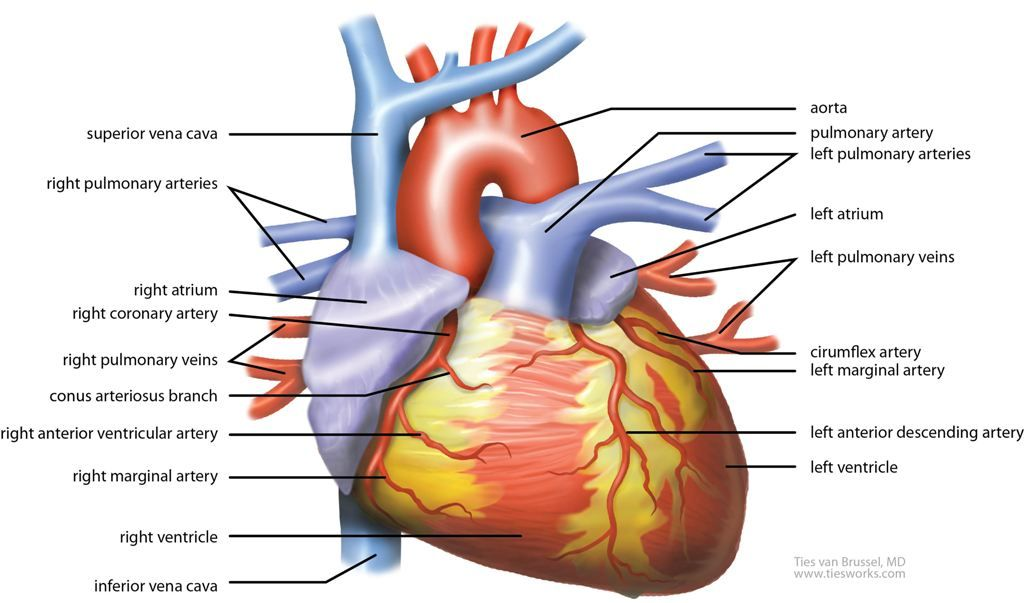
\includegraphics[width=5in]{./kap_syk/bilder/hjertebedre.jpg}}
                      \caption{Et hjerte}
                      %{Her ser vi et hjerte som er fiksert i formalin.}%\textit{tjenestetilbudene}.]
                    \end{figure}    


				%!!! Her må et bilde inn
			\paragraph{Effektiv jobbing\\}
				Når hjertet pumper med vanlig frekvens er det veldig effektivt. Da sørger det for jevn transport av blodet på en mest mulig energieffektiv måte. Når hjerteslagene blir veldig raske blir hjertet mindre effektivt\cite{FA-saladin}. Man kan kalle det en funksjonell hjertesvikt. Det betyr at hjertet er friskt, men jobber på- eller over grensen for at blodet skal strømme fritt.
				%legg inn video an ultralyd ecco cor!!!
		\section{Fysiologi}	
			\paragraph{Hva menes med hjerte- og karsykdommer?\\}\label{sec:athero}
				Som alle organer i kroppen har hjertet sine egne blodårer. De er ekstra utsatt for åreforkalking, eller atherosklerose som det heter på latin. Atherosklerose er kalkinnlagring i blodåreveggen som gjør den stiv og samtidig klumpete på innsiden. Dette hindrer blodgjennomstrømningen. Mengden med kalk i blodårene er varierende gjennom livet, men fet mat, høyt blodtrykk og sigaretter gjør at mer kalk lagres. 
		\section{Patologi}	
			\paragraph{Skader oppstår\\}
				Noen steder blir blodpassasjen dårlig og det kan dannes skader fordi vevet ikke får nok oksygen. Hjertet er en muskel med innebygget nervesystem og noen ganger blir det små skader som gror til arr i forkammeret. Dette kan skape atrieflimmer\cite{!!!}. Hvis blodårene tetter seg rundt hjertekammeret får man ofte anginasmerter, og dersom blodåren blir helt tett er det et infarkt.
		\section{Klinikk}
			\subsection{Hjerteinfarkt}	
				\paragraph{Symptomer\\}
					Trykkende smerte i brystet, utstråling til venstre arm eller underkjeve. Blek og kaldsvett, klam og tungpusten. Dette er noen klassiske symptomer ved hjerteinfarkt. Vi må passe oss fordi, eldre, pasienter med diabetes eller kvinner har ofte helt andre symptomer. 
				\paragraph{Førstehjelp\\}
					Ring ambulansen, vær hos pasienten. Gi oksygen og Dispiril hvis dere har. 
				\paragraph{Farlige momenter\\}
					De som dør av hjerteinfarkt får ofte akutt hjertflimmer. Dette er ikke atriflimmer, men kammerflimmer og er helt forskjellig. Hjertet slår med 300 slag i minuttet. Pasienten er bevisstløs og den eneste redningen er å bruke hjertestarter og å gjøre hjerte- lungeredning. Det viktigste for akutte hjerteinfarkt er rask behandling med utblokking og innsetting av stent. Noen pasienter egner seg ikke for dette, særlig de eldste og sykeste ville ikke overleve behandlingen og blir heller behandlet på sykehus uten utblokking. 
				\paragraph{Hva skjer etterpå?\\}
					Alle pasienter som har hatt hjerteinfarkt får nesten samme type medisiner:
					\begin{itemize}
						\item Metoprolol(SelZok \textregistered), gjør at hjertet for "hvile". Forebygger nye infarkt og hjerterytmeforstyrrelser. Senker blodtrykket, og gjør at makspulsen blir lavere ved fysiske anstrengelser. Noen menn blir impotente. Kalles også "Betablokker"\\
						\item Acetylsalisylsyre(Albyl-E\textregistered) \\
						\item ACE- hemmer(Renitec \textregistered) eller AT\textsubscript{2}-antagonister(Cozaar \textregistered, eller andre), senker blodtrykket.\\
						\item Statiner(Simvastatin, Atorvastatin(Lipitor\textregistered)), senker farlig kolesterol og stabiliserer crispy blodårer.\\
					\end{itemize}
				\paragraph{Tips for hverdagen\\}
					Hjertesyke pasienter bør man passe på brå endringer i tilstanden, dette gjelder forøvrig alle andre sykdomstilstander som blir beskrevet her. Hvis en pasient har kjent hjertesykdom og lav "blodprosent" kan den lave blodprosenten utløse infarkt.
			\subsection{Hjertesvikt}
				Er oftest en komplikasjon etter et hjerteinfarkt som ikke ble behandlet i tide. New York Heart Assosiation(NYHA) har klassifisert hjertesvikt etter hvordan pasientene fungere i hverdagen. 
					\begin{table}[ht]
						\caption{NYHA(New York heart assosiation) klassifisering av hjertesvikt}
						\centering
						\rowcolors{1}{cyan}{white}
						\begin{tabular}{|p{2cm}| p{11cm}|}
							\hline
							\textbf{KLASSE} & \textbf{Symptomer}\\[0.75pt]
							\hline
							1 (I) & Hjertesvikt uten kliniske symptomer\\
							\hline
							2 (II) & Hjertesviktsymptomer (dyspné, takykardi, tretthet) kun ved\newline større fysiske anstrengelser som rask gange i motbakke. \newline Pasienten kan gå 2–3 etasjer i trapp sammenhengende\\
							\hline
							3 (III) & Symptomer ved moderat fysisk anstrengelse som dagliglivets aktiviteter,\newline rolig gange på flat vei eller gange opp en etasje i trapp\\
							\hline
							4 (IV) & Symptomer i hvile eller ved minimal aktivitet som personlig stell \\
							\hline
						\end{tabular}
					\end{table}
				\paragraph{Symtomer\\}
					Tungpust og hovne bein. Slapphet og trettbarhet. Dårlig matlyst.
				\paragraph{Hva må helsepersonell passe på\\}
					Følg med på vekten. En hjertesviktpasient kan gå opp i vekt med flere kilo om dagen dersom medisinene slutter å fungere. 
				\paragraph{Hvor farlig er det\\}
					Jo høyere grad hjertesvikt jo dødligere er det. En alvorlig hjertesvikt er å sammenligne med kreftsykdommer med spredning. Ikke glem å rådføre med lindrende avdeling når det gjelder disse pasientene.
				\paragraph{Tips for hverdagen\\}
					Ikke glem å veie hjertesviktpasienter. Alle med hejrtesvikt bør føre drikkeskjema fordi for mye drikke kan forverre symptomene. 
			\subsection{Atrieflimmer}
				Noen ganger utvikler hjertet en feil i det elektriske systemet. Dette fører til atrieflimmer, som ofte kommer anfallsvis. Når blodet utsettes for ujevne hjerteslag kan det klumpe seg og føre til hjerneslag.
				\paragraph{Symptomer\\}
					Samme som hjertesvikt, men kommer ganske akutt. Pulsen er ujevn og rask. 
				\paragraph{Hva må hjemmetjenesten være oppmerksomme på?\\}
					Å drikke lite gjør at pasientene kan få anfall. Hvis blodfortynningen ikke er tilstrekkelig, vil pasientene kunne få slag. Derfor er det viktig å følge med på INR. 
				\paragraph{Medisiner\\}
					Metoprolol begrenser hjerterytmen og forebygger anfall. Marevan forebygger hjerneslag. Noen nye behandlinger er under innføring for eksempel Rivaroxiban (Xarelto\textregistered), som også virker blodfortynnende. Noen pasienter får Digitalis(Digoxin \textregistered, Digitoxin \textregistered, som det står mer om i neste kapittel.
			\subsection{Digitalis}
				Digitalis er et naturprodukt som er veldig giftig. Det styrker hjertemuskelens evne til å slå og stabiliserer hjerterytmen.
				\paragraph{Litt om farmakologi\\}
					Terapeutisk bredde betyr at man har lite spillerom med dosen til et legemiddel. Det vil si at en liten økning i dosen kan være farlig eller dødelig. \\
					Halveringstid: Betegner hvor lenge et legemiddel bruker på reisen gjennom kroppen.\\
				\paragraph{Load and go...\\}
					Digitalis har smal terapeutisk bredde, og treg passasje gjennom kroppen. Det betyr at selv ved små økninger i dosen er det lett å bli forgiftet. Det tar også lang tid å få digitalis ut av systemet, ofte flere uker dersom man har hatt for høy dose lenge. Digitalis trenger også en loading dose ved oppstart. Det betyr at en høyere dose gis ofte de første dagene for å få effekt.
				\paragraph{Rare symptomer\\}
					Fordi digitalis er lett å overdosere skjer det nokså ofte, men oppdages også sent. Det er fordi symptomene er vanskelige å skille fra andre tilstander. Kvalme, diaré og forvirring er ikke uvanlig hos eldre, men akkurat disse tre er typisk for forgiftning med Digitalis.
				\paragraph{Praktisk råd:\\}
					Hvis en pasient bruker digitalis og får diaré bør lege kontaktes. Det kan skyldes forgiftning. Husk at diaré også kan føre til at Digitalis kan bli tatt opp annerledes i kroppen.
		\section{Pasienteksempler}
			\subsection{Pasient 1}
			\subsection{Pasient 2}



\newpage